\section{Results}

\subsection{Assessment of data preprocessing methods}

% \item Considering rapid real-time interaction,
% what are the performance bottlenecks of
% an interactive web map application,
% and what data preprocessing and simplifying approaches
% are needed to overcome them?
The preprocessing parameters used for
processing the TTM for the finished map application were
a 15-minute isochrone interval and a 60-minute travel time limit.
I reduced the coordinate precision as much as
was possible without impacting the map visually.
This meant a coordinate precision of 5 decimal places,
reduced from the 15-decimal-place GeoJSON default \parencite{geojsonspec}.
File minimizing consisted of removing all whitespace from the GeoJSON files
and applying maximum gzip compression.
Preprocessing the data with these parameters
enabled a responsive enough presentation for exploring all travel modes
with both modes of interaction,
but still kept the map informative, at least from a macro-scale perspective.

Assessing these methods in more detail,
the aggregation of travel time values into 15-minute isochrone polygons was the most
effective method when it came to increasing the responsiveness of the map:
Without the isochrone approach,
the hovering mode would not have been realistic to implement.
However, 15-minute isochrone polygons also
reduced the amount of information on the map greatly,
making detail-oriented analysis of the mapped phenomenon impossible.
Limiting the spatial extent of data based on travel time also had a noticeable effect
in both the responsiveness and information loss,
but its was more dependent on the travel mode.
On slower modes of travel, for example walking,
a travel time maximum of 60 minutes resulted in
much more data being left out than on a travel mode like public transportation or car.
Likewise, the gain in responsiveness was larger on slower travel modes.
When reasoning about the performance bottleneck of the map application,
it should be noted that both these methods
reduced the geometrical complexity of the data greatly,
but also, as a result, affected file-sizes.

Limiting coordinate precision and minimizing the GeoJSON files
reduced the file sizes,
but neither method had a visible effect on map responsiveness.
These methods, with the parameters applied here,
did not result in any information loss on the map,
and did not alter the geometrical complexity of data.

In general, the methods with the most geometrical simplification
resulted in the largest gains in the responsiveness of the map,
while methods focused solely on file sizes did not affect responsiveness.
Given this, in the context of this web map application,
the geometrical complexity of data was the performance bottleneck --
file minimizing alone was not enough for enabling real-time interaction.

See table \ref{tab:preprocessing methods} for
an overview of the assessment of preprocessing methods.

\begin{table}[H]
	\caption{
		The assessment of the preprocessing methods.
		The methods applying the highest levels of geometrical simplification
		resulted in the largest increases in map responsiveness,
		but also resulted in significant information loss when mapping the data.
	}
	\label{tab:preprocessing methods}
	\centering
	\begin{tabular}{ | L{0.25\textwidth} | L{0.33\textwidth} | L{0.33\textwidth} | }
		\hline
		\textbf{Method, type of optimization}
		& \textbf{Increase in responsiveness of the map}
		& \textbf{Loss of information on the map}
		\\
		\hline
		\hline
		Aggregation into isochrone polygons (15-minute interval),
		\textit{Reducing geometrical complexity and file sizes}.
		& Large: The isochronal approach is what makes the real-time interaction possible.
		& Large: 15-minute isochrone polygons allow for quick overview
		but make detailed assessment impossible.
		\\
		\hline
		Limiting the maximum travel time (60 minutes),
		\textit{Reducing geometrical complexity and file sizes}.
		& Noticeable on all travel modes, as the largest isochrone polygons are more costly to render.
		The more data was discarded, the larger the increase:
		most increase observed when mapping the slowest travel modes.
		& Depends on travel mode:
		For walking a limit of 60 minutes means that, on average,
		the isochrones cover 3\% of the total area of the dataset.
		For cycling 30\%, for public transit 27\%, for car 98\%.
		For a given grid cell the averaged coverage of all modes is 40\%.
		\\
		\hline
		Limiting coordinate precision,
		\textit{Reducing file sizes}.
		& Potentially noticeable with limited download speeds:
		Reducing the precision of geometries reduced file sizes by 50\% on average,
		thus enabling faster data transfer.
		No visible effect on responsiveness was observed in this study.
		& None: The decreased precision is in no way visible.
		\\
		\hline
		Minimizing files by simplifying GeoJSON structure and compressing using gzip,
		\textit{Reducing file sizes}.
		& Potentially noticeable with limited download speeds:
		This reduces file sizes by 60\% on average,  % TODO
		thus enabling faster data transfer.
		No visible effect on responsiveness was observed in this study.
		& None: These approaches do not affect the content of the data.
		\\
		\hline
	\end{tabular}
\end{table}



\subsection{Assessment of mapping libraries}

% \item Visual quality of the map
% \item Responsiveness of the map
% \item UI integration capabilities (tested only with React)

Considering its visual quality,
the map contained two main aspects to assess:
The base map and the isochrone polygons drawn on top of it.
When assessing the base map,
Deck.gl and Maplibre were essentially equal as both utilized vector base maps.
This meant seamless zooming and less noticeable base map loading.
Leaflet natively uses raster base maps, which resulted in brief yet noticeable
blurring when the map is zoomed and a more detailed raster is being fetched.
When assessing the rendering of the polygons,
I observed Leaflet and Maplibre producing consistent results,
while Deck.gl produced some inconsistent visual output \parenfig{bug}.
Upon further investigating this together with the Deck.gl maintainers,
the rendering error was reproduced and proven to indeed be an issue with the library \parencite{deckbug} --
More specifically, in its underlying triangulation algorithm \parencite{earcutbug}.

\begin{figure}[H]
	\centering
	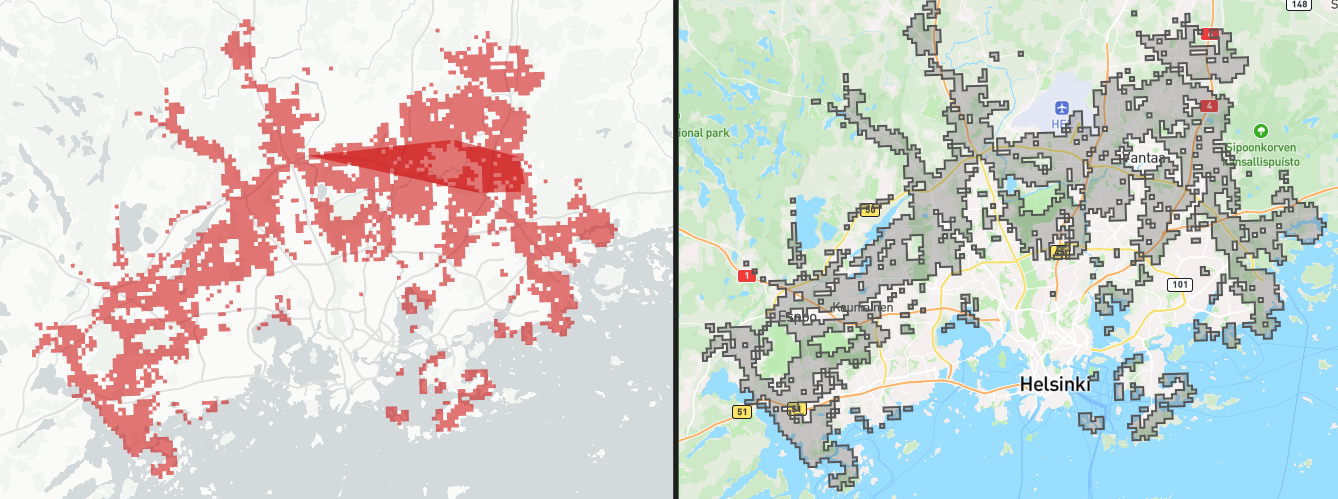
\includegraphics[width=\textwidth]{visual/figures/screenshots/bug.png}
	\caption{
		Visual artefacts were occasionally present
		when rendering complex polygons using Deck.gl.
		Here, the same isochrone polygon is rendered using Deck.gl (left)
		and a web based GeoJSON preview tool geojson.io (right).
	}
	\label{fig:bug}
\end{figure}

When assessing the responsiveness of the map interface,
Deck.gl and Maplibre were very similiar.
While both enabled real-time interaction with the map,
I observed Deck.gl to be slightly more responsive when using the hover mode,
i.e. the most computationally demanding mode of interaction.
Leaflet was not tested to the same extent here,
as the map perfofmance degraded noticeably
even when rendering only the base grid of the dataset.
Both Deck.gl and Maplibre utilized WebGL GPU acceleration,
while Leaflet did not.

All libraries had some way of integrating with React.
Deck.gl provided native integration,
meaning no additional wrapper library was needed,
and React integration did not affect the map function.
Leaflet and Maplibre both had wrapper libraries for
integrating to React applications.
Integrating Leaflet and React using React Leaflet has previously
been observed to produce performance issues \parencite{gaj2023}.
Thus, the performance issues I observed with Leaflet could be an issue of
the wrapper library instead of the mapping library itself.
Integrating Maplibre into React with React Map GL
produced a functional map application,
without issues in the development process.

For an overview of the assessment of mapping libraries,
see table \ref{tab:map library comparison}.


\begin{table}[H]
	\caption{Comparison of mapping libraries}
	\label{tab:map library comparison}
	\centering
	\begin{tabular}{ | L{0.1\textwidth} | L{0.25\textwidth} | L{0.25\textwidth} | L{0.25\textwidth} | }
		\hline
		Library
		& Quality of visualization
		& Rendering performance
		& Integration with React
		\\ 
		\hline
		\hline
		Deck.gl
		& Inconsistent rendering of complex polygons, vector tiles supported
		& GPU accelerated (WebGL), most performant of the tested libraries
		& Designed from ground up to work with React
		\\
		\hline
		Leaflet
		& Correct rendering of polygons, Vector tiles possible through plugins
		& No GPU acceleration, least performant of the tested libraries
		& Integration possible with a 3rd party wrapper
		\\
		\hline
		Maplibre
		& Correct rendering of polygons with very rare inconsistencies, vector tiles supported
		& GPU accelerated (WebGL), slightly less performant than deck.gl
		& Integration possible with a 3rd party wrapper
		\\
		\hline
	\end{tabular}
\end{table}


\subsection{Survey on map use}

(Response plots in appendices)

Most map users preferred as dynamic as possible interaction with the map,
using the most dynamic mode of interaction when given the choice.
This was the case regardless of the task type (figures \ref{fig:task 4} and \ref{fig:task 5}).

Map users rated selection of travel mode as the most useful way of
interacting with the map (figure \ref{fig:general questions}).
Hovering mode was the second most useful functionality,
and the clicking mode third.

Map interaction did affect how map users perceived the mapped phenomenon.
Most users perceived the accessibility of a location differently depending
on the mode of interaction used (figures \ref{fig:task 2} and \ref{fig:task 3}).

However, most map users did not feel like the map affected
their understanding of accessibility (figure \ref{fig:general questions}).
Those that did, mentioned:

\begin{itemize}
	\item Gaining new insight on the accessibility of different locations (n = 6)
	\item Gaining new insight on the differences between travel modes (n = 4)
	\item Understanding accessibility differently in general (n = 3)
	\item Understanding the city structure differently (n = 1)
\end{itemize}

Overall, the responses indicate that the map worked,
both in the sense of usability and conveying information about the mapped phenomenon.

